Climate change is a well-documented phenomenon: on average, the global temperature is increasing. In this section, we test the hypothesis that temperature increases in Salt Lake City and Rye Patch Dam are not equal.

Temperature anomaly is used to compare change in temperature over time. A mean temperature is calculated over a long period of time, and this long-term mean is subtracted from more recent observations. For example, it is known that the global average temperature was $13.9^{\circ}$C between 1901 and 2000. If the global average temperature in 2015 was $14.5^{\circ}$C, then the temperature anomaly for that year would be $14.5 - 13.9 = 0.6^{\circ}$C. When analyzing temperature data over many years, it is advisable to use a temperature anomaly rather than absolute temperature because it eliminates seasonal variation within the year, allowing for a more significant result. This is an accepted and widely used method in climate analysis \textcolor{red}{[DOES THIS CITATION WORK??]} \cite{temp_anomaly}

The GSOM records the monthly average temperature at each location, so we determined temperature anomaly monthly. We calculated a January anomaly by averaging the January temperatures of each year from 1948 to 1974. Then, we subtracted this long-term mean from each January temperature from 1975 to 2020. We did the same for the other eleven months and for both locations, yielding different anomalies for each. In our data files, this is column CG, labeled TAVG ADJ. We used this anomaly in our comparison in place of the absolute temperature. It served to reduce the variance of each sample to produce a meaningful result.

Because of the large number of observations in each sample, we invoked the central limit theorem to approximate the distribution as normal. The Shapiro-Wilk test for normality gives a p-value of .01663 for the Salt Lake City sample and 0.0003392 for the Rye Patch Dam sample, which verifies that the normal approximation is appropriate ($P < 0.05$). The linear nature of the plots further supports our approximation.

Formally, our hypotheses are: $$ H_{0}: \mu_{SLC} = \mu_{RPD} \;\; vs. \;\; H_{a}: \mu_{SLC} \neq \mu_{RPD}.$$ Because the two stations have similar geographical characteristics (i.e. latitude, longitude, and elevation), we determined that this is an observational matched pairs analysis and used the paired t-test at $\alpha = 0.05$ accordingly. As such, it was not necessary to determine equality of variance between the two samples. We determined the test statistic to be $t = -16.46$. This is less than the critical value $-t_{n-1,\alpha/2} = -1.648$ (where n = 487). Also, the p-value is $2.2 \times 10^{-16}$, which is less than the significance level $\alpha = 0.05$. Based on these results, we reject $H_{0}$ and conclude that the mean temperature anomaly at Salt Lake City is significantly greater than the mean temperature anomaly at Rye Patch Dam. In other words, since 1975, the temperature has increased more at Salt Lake City than at Rye Patch Dam. The reason for this is not known, but previous research suggests that Salt Lake City emits a relatively large amount of carbon pollution per capita, which hastens the effects of climate change there \cite{obama_report}. These results, and useful statistics, are summarized in Tables \ref{tab:temp_diffs} and \ref{tab:t_test_results}.

\begin{table}[ht]
 \begin{centering}
 \begin{tabular}{|c|c c|} 
 \hline
 $$ & $\Delta T$ Salt Lake City & $\Delta T$ Rye Patch \\ [0.5ex] 
 \hline\hline
  $\mu$ & 1.1229 & 0.1317 \\ 
 \hline
 $\sigma$ & 1.9765 & 1.9226 \\
  \hline
 $n$ & 487 & 487 \\ 
  \hline
 $P_{Shapiro}$ & 0.0166 & 0.0003 \\ 
 \hline
 \end{tabular}
 \caption{Temperature Difference Statistics}
 \label{tab:temp_diffs}
 \end{centering}
\end{table}

\begin{table}[ht]
 \begin{centering}
 \begin{tabular}{|c|c|} 
 \hline
  $t$ & -16.46 \\ 
 \hline
 $df$ & 486 \\
  \hline
 $P$ & $2.2 \times 10^{-16}$ \\ 
  \hline
 Conf. Interval & $(-1.1095, -0.8728)$ \\ 
 \hline
 \end{tabular}
 \caption{Paired t Test Results for $\Delta T$}
 \label{tab:t_test_results}
 \end{centering}
\end{table}

We also present the Q-Q Plots in Figures \ref{fig:slc_diff_qqplot} and \ref{fig:rp_diff_qqplot} to visualize the data normality. The linear relationships suggest that both datasets are normal.

\begin{figure}
  \centering
  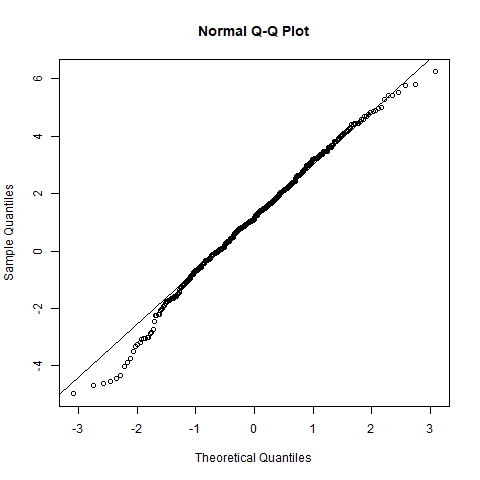
\includegraphics[width=10cm]{../data/img/Salt_Lake_Diff_QQ_Plot.PNG}
  \caption{Q-Q Plot in Salt Lake City}
  \label{fig:slc_diff_qqplot}
\end{figure}

\begin{figure}
  \centering
  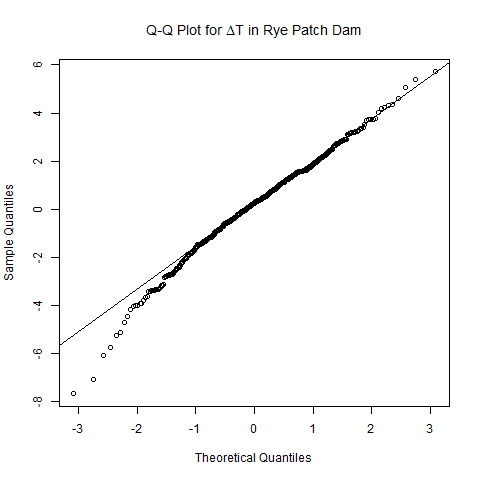
\includegraphics[width=10cm]{../data/img/Rye_Patch_Diff_QQ_Plot.PNG}
  \caption{Q-Q Plot in Rye Patch}
  \label{fig:rp_diff_qqplot}
\end{figure}

We then randomly selected 10\% of the data from each station to remove from the dataset and treat as missing. Although our dataset contains ample missing values on its own, we removed more values in order to evalued the effects of missing data. Our analysis ignored months in which temperature data for Salt Lake City \textit{or} Rye Patch Dam was missing. This resulted in a loss of total data points greater than 10\%, leaving us with a new sample size (that is different for each run) for each station. Performing the Shapiro-Wilk test again, the distribution of the observations were still normal. The new test statistic for a sample run was -13.984, which is less than the critical value  $-t_{n-1,\alpha/2} = -1.648$ (where n = 397). The p-value was $2.2 \times 10^{-16}$, which is less than the significance level $\alpha = 0.05$ (note that the reported p-value is the same as before because the true value is below machine precision). Therefore, we reject $H_{0}$ and conclude that the mean temperature anomaly at Salt Lake City is greater than the mean temperature anomaly at Rye Patch Dam. The addition of more missing values reduced the sample size and (theoretically) resulted in a higher p-value, but did not change the outcome of the hypothesis test.